\section{Константа равновесия системы $Ar-CO_2$}

\subsection*{\protect \textbf{6.1.} Константа равновесия в каноническом ансамбле \cite{keszei, landau2}}
\addcontentsline{toc}{subsection}{\protect\numberline{6.1} Константа равновесия в каноническом ансамбле}

Канонический ансамбль представляет собой модель термодинамической системы, погруженной в тепловой резервуар постоянной температуры. В представленной системе резервуар играет роль термостата, поддерживая температуру исследуемой системы постоянной независимо от направления теплового потока. Канонический ансамбль (также называемый $NVT$-ансамблем) представляет собой систему из $N$ частиц, находящихся в фиксированном объеме $V$ при фиксированной температуре $T$. Отметим, что энергия $NVT$-ансамбля может принимать любые значения, согласующиеся с заданными условиями. Рассматривая совокупность резервуара и погруженной в него исследуемой системы как микроканонический ансамбль, получают каноническое распределение (распределение Гиббса) -- вероятность нахождения системы в состоянии с энергией $E_n$:
\vverh
\begin{gather}
	\omega_n = A \times \exp \lb - \frac{E_n}{kT} \rb \quad \Leftrightarrow \quad \rho \lb p, q \rb = A \times \exp \lb - \frac{E \lb p, q \rb}{kT} \rb \notag
\end{gather}
Энтропия может быть выражена как среднее значение функции распределения:
\vverh
\begin{gather}
	S = - \langle \ln \omega_n \rangle \notag \\
	S = - \ln A + \frac{1}{T} \langle E_n \rangle = - \ln A + \frac{\overline{E}}{kT} \notag \\
	\ln A = \frac{\overline{E} - TS}{kT} = \frac{F}{kT} \notag 
\end{gather}
Средняя энергия $\overline{E}$ есть как раз то, что понимается в термодинамике под энергией $U$, таким образом получаем следующее выражение для функции распределения Гиббса через свободную энергию Гельмгольца (в квантовой и классической статистиках, соответственно):
\vverh
\begin{gather}
	\omega_n = \exp \lb - \frac{F - E_n}{kT} \rb \quad \Leftrightarrow \quad \rho(p, q) = \frac{1}{\lb 2 \pi \hbar \rb^{s}} \exp \lb \frac{F - E(p, q)}{kT} \rb \notag
\end{gather}

Условие нормировки для распределения $\omega_n$:
\vverh
\begin{gather}
	\sum_n \omega_n = \exp \lb \frac{F}{kT} \rb \sum_n \exp \lb - \frac{E_n}{kT} \rb = 1 \notag \\
	F = - kT \ln \sum_n \exp \lb - \frac{E_n}{kT} \rb = - kT \ln Z \notag
\end{gather}

При записи аналогичной формулы в классической термодинамике следует учесть, что если, например, переменить местами два одинаковых атома, то после такой перестановки микросостояние тела будет изображаться другой фазовой точкой, получающейся из первоначальной заменой координат и импульсов одного атома координатами и импульсами другого. С другой стороны, ввиду одинаковости переставляемых атомов, оба состояния тела физически тождественны. Таким образом, одному и тому же физическому микросостоянию тела в фазовом пространстве соответствует целый ряд точек. При интегрировании распределения каждое состояние должно учитываться лишь однократно (статистический интеграл можно рассмотреть как предел квантовой статистической суммы, суммирование в которой производится по всем различным квантовым состояниям), то есть интегрирование производится лишь по тем областям фазового пространства, которые соответсвуют физически различным состояниям тела (штрих над интегралом будет подчеркивать эту особенность классической статистической суммы).
\vverh
\begin{gather}
	F = -k T \ln \int^{\prime} \exp \lb - \frac{E(p, q)}{kT} \rb d \Gamma, \quad d \Gamma = \frac{dp \, dq}{\lb 2 \pi \hbar \rb^s} \notag
\end{gather}

Запишем свободную энергию Гельмгольца, используя молекулярную статистическую сумму $q$. (Слагаемое $F(0)$ призвано подправить значение в правой части равенства, что существенно в силу свободы выбора начала отсчета для молекулярной суммы по состояниям.)  
\vverh
\begin{gather}
	F = - k T \ln Q = F(0) - kT \ln \frac{q^N}{N!} = F(0) - NkT \ln q + NkT \lb \ln N - 1 \rb \notag 
\end{gather}

Полагая $N = N_A$, приходим к мольному значению свободной энергии Гельмгольца:
\vverh
\begin{gather}
	F_m = F_m(0) - RT \ln \frac{q}{N_A} - RT \notag
\end{gather}

В приближении идеального газа имеем $G_m = F_m + p V_m = F_m + RT$. Заметим, что $F_m(0) = U_m(0)$. Под $q^{\barcirc} = q_{NVT}^{\barcirc}$ понимается значение суммы по состояниям, вычисленное при $N = N_A$, фиксированной температуре $T$ и при фиксированном объеме $V = \frac{RT}{p^{\barcirc}}$.
\vverh
\begin{gather} 
	G_m = F_m(0) - RT \ln \frac{q}{N_A} \notag \\
	G^{\barcirc} = U_m(0) - RT \ln \frac{q^{\barcirc}}{N_A} \notag \\
	\Delta_r G^{\barcirc} = \Delta_r U_m(0) - RT \ln \prod_{i} \lb \frac{q_i^{\barcirc}}{N_A} \rb ^{\nu_i} \notag
\end{gather}

Используя равенство $\Delta_r G^{\barcirc} = - RT \ln K$, получаем выражение для термодинамической константы равновесия:
\vverh
\begin{gather}
	K = \prod_{i = 1}^{r} \lb \frac{q_i^{\barcirc}}{N_A} \rb^{\nu_i} \exp \lb - \frac{\Delta_r U_m (0)}{RT} \rb \notag
\end{gather}

Термодинамическая и газовая константы равновесия связаны между собой следующим соотношением: 
\vverh
\begin{gather}
	K_p =  K \times \lb p^{\barcirc} \rb^{\sum_i \nu_i} \notag 
\end{gather}

Получим выражение для газовой константы равновесия $K_p$ слабосвязанного комплекса $Ar-CO_2$. В условиях совпадающего начала отсчета молекулярных сумм по состояниям для всех участников реакции получаем следующее выражение:
\vverh
\begin{gather}
	K_p = \frac{N_A}{p^{\barcirc}} \frac{q_{Ar-CO_2}^{\barcirc}}{q_{Ar}^{\barcirc} q_{CO_2}^{\barcirc}} \label{eqconst}
\end{gather}

\subsection*{\textbf{6.2.} Статистическая сумма связанного димера} 
\addcontentsline{toc}{subsection}{\protect\numberline{6.2} Статистическая сумма связанного димера}

Связанным димером называют такое состояние пары мономеров, при котором энергия меньше, чем у мономеров, разведенных на бесконечно большое расстояние. Классическая сумма по состояниям связанного димера представляет собой следующий фазовый интеграл
\vverh
\begin{gather}
	Q_{bound}^{pair} = \frac{1}{h^8} \int\limits_{H - \ddfrac{\strut P_{cm}^2}{\strut 2 M} < 0} \exp \lb - \frac{H}{k T} \rb d x_{cm} d y_{cm} d z_{cm} d P_{x} d P_{y} d P_{z} d q_i d p_i, \label{ci1}
\end{gather}

где $q_i$, $p_i$ -- набор внутримолекулярных координат и импуьсов, $H$ - гамильтониан, записанный в лабораторной системе координат, $\mathbf{R} = \lb x_{cm}, y_{cm}, z_{cm} \rb$, $\mathbf{P}_R = \lb P_x, P_y, P_z \rb$ -- векторы координат и импульсов центра масс, а $M$ -- его масса. \par
Отметим, что гамильтониан, фигурирующий в выражении \eqref{ci1}, связан с гамильтонианом в молекулярно-фиксированной системе отсчета соотношением
\vverh
\begin{gather}
	H = \mH + \frac{P_{cm}^2}{2 M} \notag
\end{gather}

Интегрирование по векторам центра масс $\mf{R}$, $\mf{P}_R$ в выражении \eqref{ci1} дает трансляционную сумму по состояниям димера:
\vverh
\begin{gather}
	\lb Q_{bound}^{pair} \rb_{tr} = \lb \frac{2 \pi M k T}{h^2} \rb^{\frac{3}{2}} V \notag
\end{gather}

\subsection*{\textbf{6.3.} Эйлеровы углы и сопряженные им импульсы}
\addcontentsline{toc}{subsection}{\protect\numberline{6.3} Эйлеровы и сопряженные им импульсы}

Рассмотрим кинетическую энергию в лагранжевой форме
\vverh
\begin{gather}
	T_\mL = \frac{1}{2} \dot{\mf{q}}^\top \bba \, \dot{\mf{q}} + \mf{\Omega}^\top \bbA \dot{\mf{q}} + \frac{1}{2} \mf{\Omega}^\top \bbI \, \mf{\Omega} \notag
\end{gather}
Вектор угловой скорости $\mf{\Omega}$ связан с вектором эйлеровых скоростей $\dot{\mf{e}}$ при помощи матрицы $\bbV$ \cite{goldstein}:
\begin{gather}
\mathbf{\Omega} = \mathbb{V} \dot{\mathbf{e}} = 
\begin{bmatrix}
\sin \theta \sin \psi & \cos \varphi & 0 \\
\sin \theta \cos \psi & - \sin \psi & 0 \\
\cos \theta & 0 & 1
\end{bmatrix}
\begin{bmatrix}
\dot{\varphi} \\
\dot{\theta} \\
\dot{\psi}
\end{bmatrix} \notag 
\end{gather}

По определению построим вектор эйлеровых импульсов:
\vverh
\begin{gather}
	\mf{p}_e = \frac{\partial T_\mL}{\partial \dot{\mf{e}}} = \bbV^\top \bbA \dot{\mf{q}} + \bbV^\top \bbI \, \bbV \dot{\mf{e}} = \bbV^\top \bbA \dot{\mf{q}} + \bbV^\top \bbI \, \mf{\Omega} \notag
\end{gather}

Несложно показать, что вектор углового момента в подвижной системе отсчета равен
\vverh
\begin{gather}
	\mf{J} = \frac{\partial \mL}{\partial \mf{\Omega}} = \bbA \dot{\mf{q}} + \bbI \, \mf{\Omega} \notag
\end{gather}

Таким образом, получаем следующую связь между вектором эйлеровых импульсов и вектором углового момента:
\vverh
\begin{gather}
	\mf{J} = \lb \bbV^\top \rb^{-1} \mf{p}_e \notag
\end{gather}

Интегрирование в \eqref{ci1} в том числе ведется по эйлеровым углам и импульсам. В связи с этим рассмотрим следующий кратный интеграл и осуществим в нем замену переменных $p_\varphi, p_\theta, p_\psi \longrightarrow J_x, J_y, J_z$. (В этом подразделе $\theta$ -- один из эйлеровых углов, а не внутренняя координата системы $Ar-CO_2$. Эта замена нам интересна по той причине, что в выражение для гамильтониана входят именно компоненты углового момента, а не эйлеровы импульсы; так выражение получается намного более компактным.)
\vverh
\begin{gather}
	\int\limits_{0}^{2 \pi} d \varphi \int\limits_{0}^{\pi} d \theta \int\limits_{0}^{2 \pi} d \psi \int d p_\varphi \int d p_\theta \int d p_\psi = \int \, \left[ Jac \right] d J_x \int d J_y \int d J_z \notag
\end{gather}

Якобиан замены переменных равен
\vverh
\begin{gather}
	\left[ Jac \, \right] = \Bigg{|} \frac{\partial \mathbf{p}}{\partial \mathbf{J}} \Bigg{|} = \Bigg{|} \det \lb \bbV^\top \rb \Bigg{|} = \sin \theta \notag
\end{gather}

Если подынтегральное выражение не зависит от эйлеровых углов (как в случае со статистической суммой связанного димера), то интегральное выражение преобразуется к виду
\vverh
\begin{gather}
	\int\limits_{0}^{2 \pi} d \varphi \int\limits_{0}^{\pi} d \theta \int\limits_{0}^{2 \pi} d \psi \int d p_\varphi \int d p_\theta \int d p_\psi = 8 \pi^2 \int d J_x \int d J_y \int d J_z \notag 
\end{gather}

Однако в случае системы $Ar-CO_2$ вращение на углы $\psi$, большие $\pi$, не приводит к новым состояниям системы (из-за симметричности молекулы $CO_2$), следовательно, для рассматриваемой системы интегральное выражение имеет вид
\vverh
\begin{gather}
	\int\limits_{0}^{2 \pi} d \varphi \int\limits_{0}^{\pi} d \theta \int\limits_{0}^{\pi} d \psi \int d p_\varphi \int d p_\theta \int d p_\psi = 4 \pi^2 \int d J_x \int d J_y \int d J_z \notag 
\end{gather}

\subsection*{\textbf{6.4.} Упрощенный вид суммы по состояниям связанного димера}
\addcontentsline{toc}{subsection}{\protect\numberline{6.4} Упрощенный вид суммы по состояниям связанного димера}

Заменяя эйлеровы импульсы на компоненты углового момента и интегрируя по переменным центра масс, сводим интеграл \eqref{ci1} к следующему:
\vverh
\begin{gather}
	Q_{bound}^{pair} = \lb Q_{bound}^{pair} \rb_{tr} \frac{4 \pi^2}{h^5} \int\limits_{\mH < 0} \exp \lb - \frac{\mH}{kT} \rb d R \, d \theta \, d p_R \, d p_\theta \, d J_x \, d J_y \, d J_z. \notag
\end{gather}

Рассмотрим гамильтониан системы $Ar-CO_2$ в молекулярно-фиксированной системе координат:
\begin{gather}
	\mH = \frac{1}{2 \mu_2} p_R^2 + \lb \frac{1}{2 \mu_2 R^2} + \frac{1}{2 \mu_1 l^2} \rb p_\theta^2 - \frac{1}{\mu_2 R^2} p_\theta J_y + \frac{1}{2 \mu_2 R^2} J_y^2 + \frac{1}{2 \mu_2 R^2} J_x^2 + \frac{1}{2 \sin^2 \theta} \lb \frac{\cos^2 \theta}{\mu_2 R^2} + \frac{1}{\mu_1 l^2} \rb J_z^2 + \notag \\
+ \frac{\ctg \theta}{\mu_2 R^2} J_x J_z + U(R, \theta) \notag
\end{gather}

Заметим, что форма гамильтониана $\mH$ позволяет представить его в виде положительно определенной квадратичной формы:
\begin{gather}
	\mH = \frac{p_R^2}{2 \mu_2} + \frac{p_\theta^2}{2 \mu_1 l^2} + \frac{1}{2 \mu_2 R^2} \lb p_\theta - J_y \rb^2 + \frac{1}{2 \mu_2 R^2} \lb J_x + J_z \ctg \theta \rb^2 + \frac{J_z^2}{2 \mu_1 l^2 \sin^2 \theta} + U(R, \theta) \notag
\end{gather}

Дальнейшие преобразования основаны на анализе фазового интеграла, представленном в работе \cite{vigasin2015}. Подготовим следующую линейную замену переменных $p_R, p_\theta, J_x, J_y, J_z \rightarrow x_1, x_2, x_3, x_4, x_5$ (причем $R, \theta$ считаем постоянными при осуществлении замены), упрощающую подэкспоненциальное выражение (впервые предложена в \cite{ozaki1985}):
\vverh
\begin{gather}
	\hspace*{-0.5cm}
	\everymath{\scriptstyle}
	\footnotesize
	\left\{
	\begin{aligned}
	x_1^2 &= \frac{p_R^2}{2 \mu_2 kT} \\
	x_2^2 &= \frac{p_\theta^2}{2 \mu_1 l^2 kT} \\
	x_3^2 &= \frac{ \lb p_\theta - J_y \rb^2}{2 \mu_2 R^2 k T} \\
	x_4^2 &= \frac{ \lb J_x + J_z \ctg \theta \rb^2}{2 \mu_2 R^2 k T} \\
	x_5^2 &= \frac{J_z^2}{2 \mu_1 l^2 \sin^2 \theta kT}
	\end{aligned}
	\right. \quad \implies \quad 
	\left\{
	\begin{aligned}
	dx_1 &= \frac{dp_R}{\sqrt{ 2 \mu_2 k T}} \\
	dx_2 &= \frac{dp_\theta}{\sqrt{2 \mu_1 l^2 k T}} \\
	dx_3 &= \frac{dp_\theta - dJ_y}{\sqrt{2 \mu_2 R^2 k T}} \\
	dx_4 &= \frac{dJ_x + \ctg \theta dJ_z}{ \sqrt{2 \mu_2 R^2 k T}} \\
	dx_5 &= \frac{dJ_z}{\sqrt{2 \mu_1 l^2 \sin^2 \theta k T}}
	\end{aligned}
	\right. \quad \implies \quad
	\left\{
	\begin{aligned}
		dp_R &= \sqrt{2 \mu_2 k T} dx_1 \\
		dp_\theta &= \sqrt{2 \mu_1 l^2 kT} dx_2 \\
		dJ_y &= \sqrt{2 \mu_1 l^2 kT} dx_2 - \sqrt{2 \mu_2 R^2 kT} dx_3 \\
		dJ_x &= \sqrt{2 \mu_2 R^2 kT} dx_4 - \sqrt{2 \mu_1 l^2 \cos^2 \theta kT} dx_5 \\
		dJ_z &= \sqrt{2 \mu_1 l^2 \sin^2 \theta kT} dx_5
	\end{aligned}
	\right.
	\notag
\end{gather}

Для упрощения выражений откинем на время трансляционную сумму по состояниям димера и $4 \pi^2$. С учётом теоремы Фубини интеграл \eqref{ci1} может быть представлен в виде повторного интеграла, в котором сначала интегрирование ведется по переменным $p_R$, $p_\theta$, $J_x$, $J_y$, $J_z$, а затем  -- по переменным $R, \theta$. Таким образом, во внутреннем интеграле переменные $R, \theta$ являются постоянными, что позволяет осуществить приготовленную замену:
\vverh
\begin{gather}
	\frac{1}{h^5} \int_{H < 0} \exp \lb -\frac{\mH}{kT} \rb dR \, dp_R \, d \theta \, dp_\theta \, d J_x \, d J_y \, d J_z = \frac{1}{h^5} \iint dR \, d \theta \int \exp \lb -\frac{\mH}{kT} \rb d p_R \, d p_\theta \, d J_x \, d J_y \, d J_z = \notag \\
	= \frac{1}{h^5} \iint  \left[ Jac \, \right] \exp \lb -\frac{U}{kT} \rb d R \, d \theta \times \idotsint\limits_{x_1^2 + \dots + x_5^2 + \frac{U}{kT} < 0} \exp \lb - x_1^2 - \dots - x_5^2 \rb dx_1 \dots dx_5, \notag 
\end{gather}

\vlevo где якобиан замены переменных $\left[ Jac \, \right]$ равен следующему произведению радикалов: 
\begin{gather}
	\hspace*{-1.0cm}
	\left[ Jac \, \right] = \Bigg{|} \frac{\partial [p_R, p_\theta, J_x, J_y, J_z]}{\partial [x_1, x_2, x_3, x_4, x_5]} \Bigg{|} = \det  
	\begin{bmatrix}
		\sqrt{2 \mu_2 k T} & 0 & 0 & 0 & 0 \\
		0 & \sqrt{2 \mu_1 l^2 k T} & 0 & 0 & 0 \\
		0 & 0 & 0 & \sqrt{2 \mu_2 R^2 k T} & -\sqrt{2 \mu_1 l^2 \cos^2 \theta} \\
		0 & \sqrt{2 \mu_1 l^2 k T} & -\sqrt{2 \mu_2 R^2 k T} & 0 & 0 \\
		0 & 0 & 0 & 0 & \sqrt{2 \mu_1 l^2 \sin^2 \theta k T}
	\end{bmatrix} = \notag \\
	= \sqrt{2 \mu_2 k T} \sqrt{2 \mu_1 l^2 k T} \sqrt{2 \mu_2 R^2 kT} \sqrt{2 \mu_2 R^2 kT} \sqrt{2 \mu_1 l^2 \sin^2 \theta kT} = (2 \mu_2 kT)^\frac{3}{2} 2\mu_1 l^2 k T R^2 \sin \theta \notag
\end{gather}

Интеграл функции $\exp \lb - x_1^2  - x_2^2 - \dots - x_n^2 \rb$ по объему $n$-мерного шара с радиусом $R$ есть (доказательство этого соотношения приведено в приложении \eqref{appendix:multint})
\vverh
\begin{gather}
	\idotsint\limits_{x_1^2 + \dots + x_n^2 \leqslant R} \exp \lb -x_1^2 - x_2^2 - \dots - x_n^2 \rb d x_1 \dots d x_n = \pi^\frac{n}{2} \frac{\gamma \lb \frac{n}{2}, R^2 \rb}{\Gamma \lb \frac{n}{2} \rb}, \notag
\end{gather}
где $\gamma(a, b)$ -- неполная гамма-функция:
\vverh
\begin{gather}
	\gamma \lb a, b \rb = \int\limits_0^b \omega^{a - 1} \exp \lb - \omega \rb d \omega \notag
\end{gather}

Применяя общее соотношение для 5-мерного случая, получаем:
\vverh
\begin{gather}
	\idotsint\limits_{x_1^2 + \dots  + x_5^2 \leqslant -\frac{U}{k T}} \exp \lb - x_1^2 - \dots - x_5^2 \rb d x_1 \dots d x_5 = \pi^\frac{5}{2} \frac{\gamma \lb \frac{5}{2}, - \frac{U}{k T} \rb}{\Gamma \lb \frac{5}{2} \rb} \notag
\end{gather}

Итак, фазовый интеграл представлен в виде интеграла по переменным $R, \theta$ и интеграла по объему 5-мерного шара, радиус которого определяется значением потенциальной функции $U(R, \theta)$. Заметим, что радиус шара является ненулевым только при отрицательных значениях потенциальной функции $U(R, \theta)$, следовательно фазовый интеграл принимает ненулевые значения только в том случае, если переменные $R, \theta$ лежат в области $U < 0$.
\vverh
\begin{gather}
	\hspace*{-9cm} \frac{1}{h^5} \iint d R \, d \theta \int \exp \lb -\frac{\mH}{k T} \rb d p_R  \, dp_\theta \, dJ_x \, dJ_y \, dJ_z = \notag \\
	\hspace{5cm} =\lb \frac{2 \pi \mu_2 k T}{h^2} \rb^{\frac{3}{2}} \frac{2 \mu_1 l^2 \pi k T}{h^2} \iint\limits_{U < 0} \exp \lb -\frac{U}{k T} \rb \frac{\gamma \lb \frac{5}{2}, - \frac{U}{k T} \rb}{\Gamma \lb \frac{5}{2} \rb} R^2 \sin \theta dR \, d\theta \notag 
\end{gather}

Итак, выражение для статистической суммы связанного димера принимает вид:
\vverh
\begin{gather}
	Q_{bound}^{pair} = 4 \pi^2 \lb \frac{2 \pi M k T}{h^2} \rb^{\frac{3}{2}} V \lb \frac{2 \pi \mu_2 k T}{h^2} \rb^{\frac{3}{2}} \frac{2 \mu_1 l^2 \pi k T}{h^2} \iint\limits_{U < 0} \exp \lb -\frac{U}{k T} \rb \frac{\gamma \lb \frac{5}{2}, - \frac{U}{k T} \rb}{\Gamma \lb \frac{5}{2} \rb} R^2 \sin \theta dR \, d\theta \notag
\end{gather}
Заметим, что предынтегральные множители могут быть выражены через статистические суммы мономеров:
\vverh
\begin{gather}
	Q_{CO_2} = Q_{CO_2}^{tr} Q_{CO_2}^{rot} = \lb \frac{2 \pi m_{CO_2} k T}{h^2} \rb^{\frac{3}{2}} V \frac{4 \pi^2 k T}{h^2} \mu_1 l^2 \notag \\
	Q_{Ar} = Q_{Ar}^{tr} = \lb \frac{2 \pi m_{Ar} k T}{h^2} \rb^{\frac{3}{2}} \notag \\
	Q_{bound}^{pair} = 2 \pi Q_{Ar} Q_{CO_2} \iint\limits_{U < 0} \exp \lb - \frac{U}{kT} \rb \frac{\gamma \lb \frac{5}{2}, - \frac{U}{k T} \rb}{\Gamma \lb \frac{5}{2} \rb} R^2 \sin \theta d R \, d \theta \notag
\end{gather}

\subsection*{\textbf{6.5.} Расчет константы равновесия системы $Ar-CO_2$}
\addcontentsline{toc}{subsection}{\protect\numberline{6.5} Расчет константы равновесия системы $Ar-CO_2$}

Подставляя полученное выражение для статистической суммы димера в \eqref{eqconst}, получаем
\vverh
\begin{gather}
	K_p = \frac{2 \pi N_A}{R T} \iint\limits_{U < 0} \exp \lb - \frac{U}{k T} \rb \frac{\gamma \lb \frac{5}{2}, - \frac{U}{kT} \rb}{\Gamma \lb \frac{5}{2} \rb} R^2 \sin \theta d R \, d \theta \label{eqconstsimple}
\end{gather}

Расчет константы равновесия по формуле \eqref{eqconstsimple} проводился при помощи адаптивного метода Монте-Карло \cite{lepage1978, vegas}. Полученная температурная зависимость константы равновесия представлена на  Рис. \ref{fig:pic3}. Результат этого расчета использовался в дальнейшем в качестве реперного для более сложных расчетов. 
\vverh
\begin{figure}[!ht]
	\hspace*{-1.2cm}
	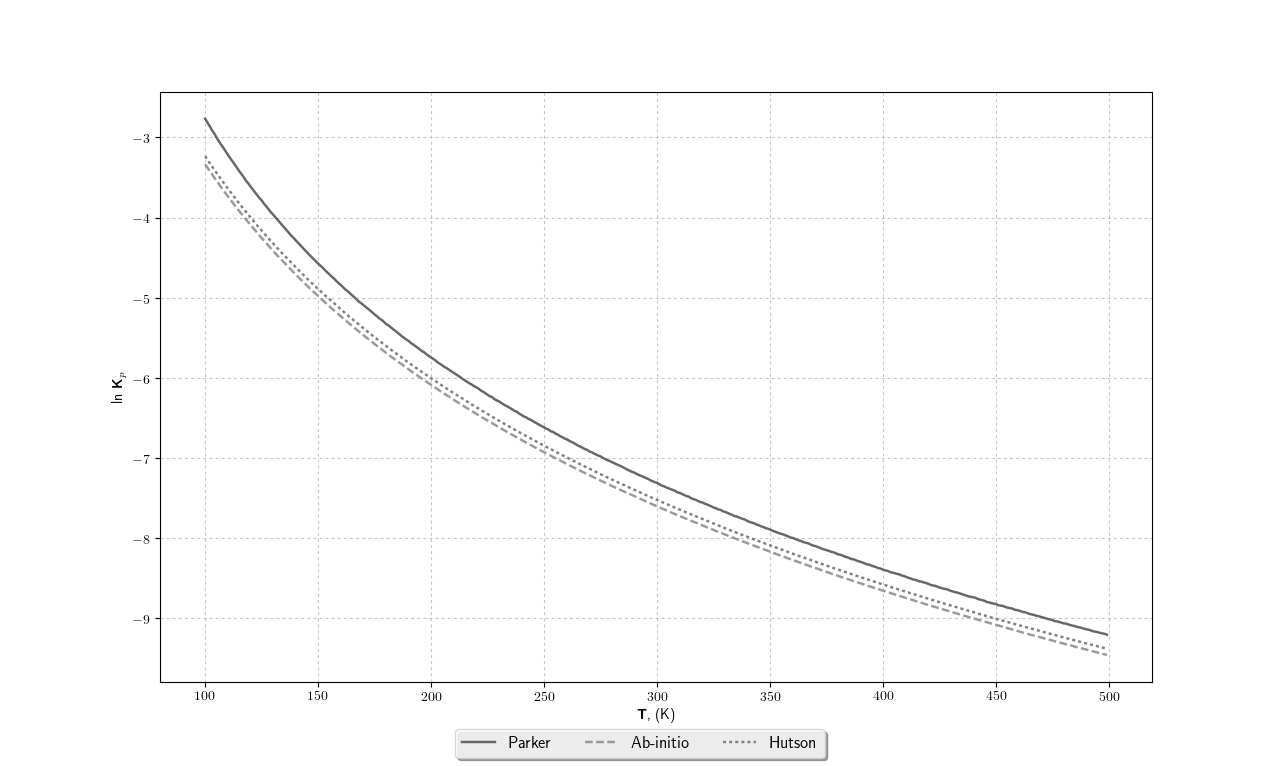
\includegraphics[width=1.1\textwidth]{pictures/all_eq_const.png}
	\caption{Зависимость логарифма константы равновесия от температуры}
	\label{fig:pic3}
\end{figure}

Следующим шагом стал расчет константы равновесия по выражению
\vverh
\begin{gather}
	K_p = \frac{4 \pi^2 N_A}{RT} \frac{ \lb Q_{bound}^{pair} \rb_{tr}}{Q_{Ar} Q_{CO_2}} \int\limits_{\mH < 0} \exp \lb - \frac{\mH}{k T} \rb d R \, d \theta \, d p_R \, d p_\theta \, d J_x \, d J_y \, d J_z \label{eqconstdim} 
\end{gather}

Расчет константы по выражению \eqref{eqconstdim} требует значительно большего компьютерного ресурса, однако позволяет рассчитывать константы равновесия для более сложных систем, для которых невозможно использовать техники, существенно уменьшающие размерность интеграла. Значения констант, получаемые этим способом, идентичны полученным по выражению \eqref{eqconstsimple}. \par 
В рамках следующего этапа мы отказались от аналитической формы гамильтониана. Расчет производился по тому же выражению \eqref{eqconstdim}, но гамильтониан $\mH$ в подынтегральном рассчитывался через матрицы $\bba, \bbA, \bbI$, определяющие лагранжиан. При вычислении значения гамильтониана в точке преобразованного фазового пространства $\left\{ R_0, \theta_0, p_{R, 0}, p_{\theta, 0}, J_{x, 0}, J_{y, 0}, J_{z, 0} \right\}$ значения $\mf{q}_{\, 0} = \left\{ R_0, \theta_0 \right\}$ используются для получения численных значений матриц $\bba_{\, 0}, \bbA_{\, 0}, \bbI_{\, 0}$. Полученные матрицы используются для численного расчета матриц $\bbG_{11, 0}, \bbG_{12, 0}, \bbG_{22, 0}$ по формулам \eqref{frob}. Затем эти матрицы используются для расчета значения гамильтониана по выражению \eqref{genham}. \par
Описанная вычислительная процедура была реализована на \textit{C++} (пакет оптимизированных процедур линейной алгебры \textit{Eigen}). Для портирования собранной процедуры на \textit{Python} была написана тонкая обертка в \textit{Cython}. Расчет многомерного интеграла осуществлялся адаптивным методом Монте-Карло \cite{lepage1978, vegas}. \par 
В результате построена вычислительная схема, позволяющая получать температурную зависимость константы равновесия по матрицам, задающим лагранжиан, для существенно более сложных систем. Данная процедура проверена на системе $Ar-CO_2$, для которой константа равновесия может быть рассчитана по существенно более простому выражению \eqref{eqconstsimple}.   

\section{Выводы}

\begin{itemize}
 \item Описан метод получения точного классического колебательно-вращательного гамильтониана. Получен точный классический колебательно-вращательный гамильтониан системы $Ar-CO_2$.
 \item Выполнен расчет температурной зависимости второго вириального коэффициента с учетом первых квантовых поправок. Расчет проведен с использованием наиболее точной поверхности потенциальной энергии, полученной в \cite{kalugina2017} методом \textit{ab initio}.  
 \item Согласно методу, развитому в \cite{vigasin2015}, выражение для константы равновесия системы $Ar-CO_2$ было сведено к двумерному интегралу по области $U < 0$. 
 \item Была построена вычислительная схема, основанная на алгоритме адаптивного интегрирования по Монте-Карло \cite{lepage1978, vegas}, позволяющая вычислять константу равновесия интегрированием по преобразованному фазовому пространству $\left\{ \mf{q}, \mf{p}, \mf{J} \right\}$, не используя упрощающих аналитических техник. 
  \item Расчет температурной зависимости константы равновесия выполнен двумя способами, и показано, что результаты этих расчетов идентичны.
\end{itemize}

